\documentclass{article}
%\documentclass[journal,transmag]{IEEEtran}
%\documentclass[10pt, conference]{IEEEtran}
\usepackage{amsmath}
\usepackage{graphicx}
%\usepackage{listings}
%\usepackage{circuitikz}
\usepackage{lscape}
\usepackage{ulem}
\usepackage{float}


\usepackage[scale=0.8]{geometry}
\begin{document}

\title{E6312: Problem Set 2}
\author{Miles Sherman}
\date{\today}
\maketitle

\textit{In the previous problem set, I measured various behaviors of the MOSFET transistor at the 180nm technology node. I mostly made direct measurements on input and output voltages as well as currents in an effort to better understand the different regions of operation of the devices. In this problem set, I take a first step towards measurement of parasitics in the devices by looking at intrinsic capacitances. In addition, I will build three basic amplifiers and measure their performance.}

\section{Problem 1: Intrinsic Capacitances}
\subsection{$C_{gs}$}
I measured the values for the gate to source capacitance using both DC operating point simulation as well as AC Analysis. To acquire the necessary DC operating simulation I first constructed the circuit shown in Figure \ref{1_dc_schem}. This circuit allows utilizes an nMOS transistor with $W/L = 1\mu m/180nm$. I ran a DC simulation on the circuit sweeping $V_{DS}$ from 0V to 1.8V and outputting drain current with $V_{GS}$ = 0.8V. Using the results browser I then plotted $C_{gs}$ against $V_{DS}$ (Figure ).

My next step was to attempt to attain the same measurements of $C_{gs}$ using the method of AC analysis. To do this, I began by constructing the circuit shown in Figure \ref{1_ac_schem} (note that the two AC voltage sources are toggled on/off in the simulating environment). My goal in this simulation was to isolate $C_{gs}$ and utilize the capacitance equation
\begin{equation}
C = \frac{i_c}{2\pi fv_c}
\end{equation}
to plot $C_{gs}$. I applied an AC signal of 10mV amplitude and low frequency to the source of the device. I then plotted the current into the gate of the device while sweeping $V_{DS}$. Even though the current at the gate flows to $C_{gs}$ and $C_{gd}$, because the AC voltage is on the source, AC current flows through $C_{gs}$ but not $C_{gd}$. Utilizing equation 1 as well as the overlap capacitance which was acquired from the results browser, I was able to plot $C_{gs}$ against $V_{DS}$ (Figure \ref{1d}). As is expected in both of my plots, $C_{gs}$ begins at approximately $C_{OX}/2$ ($C_{OX} ~= 1.5fF$), rises steadily at low values of $V_{DS}$, and saturates at approximately $\frac{2}{3} C_{OX}$ once $V_{DS} > V_{DS-SAT}$.

\begin{figure}[H]
\centering
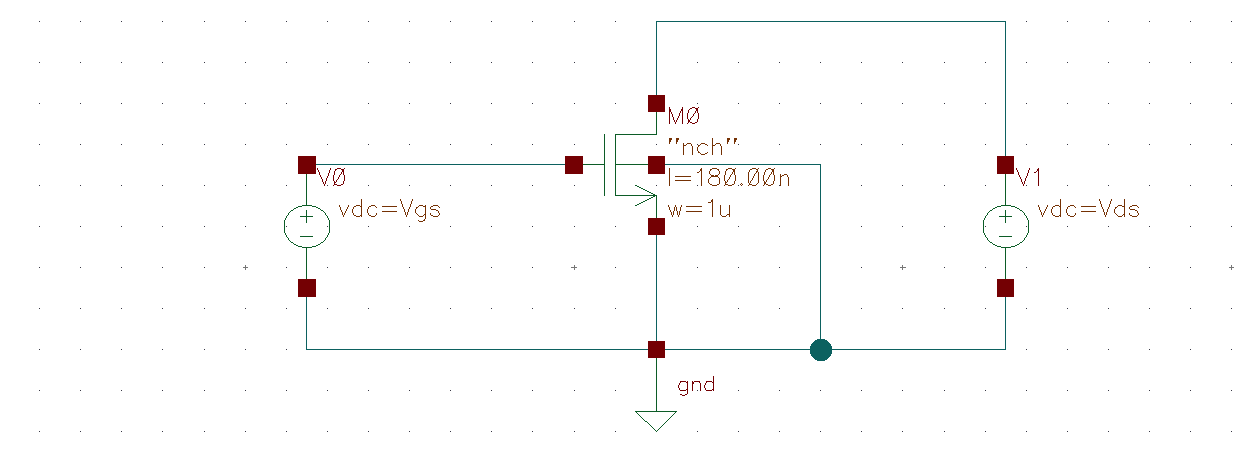
\includegraphics[width=7in]{1_dc_schematic.png}
\caption{Schematic to Simulate DC Operating Point}
\label{1_dc_schem}
\end{figure}

\begin{figure}[H]
\centering
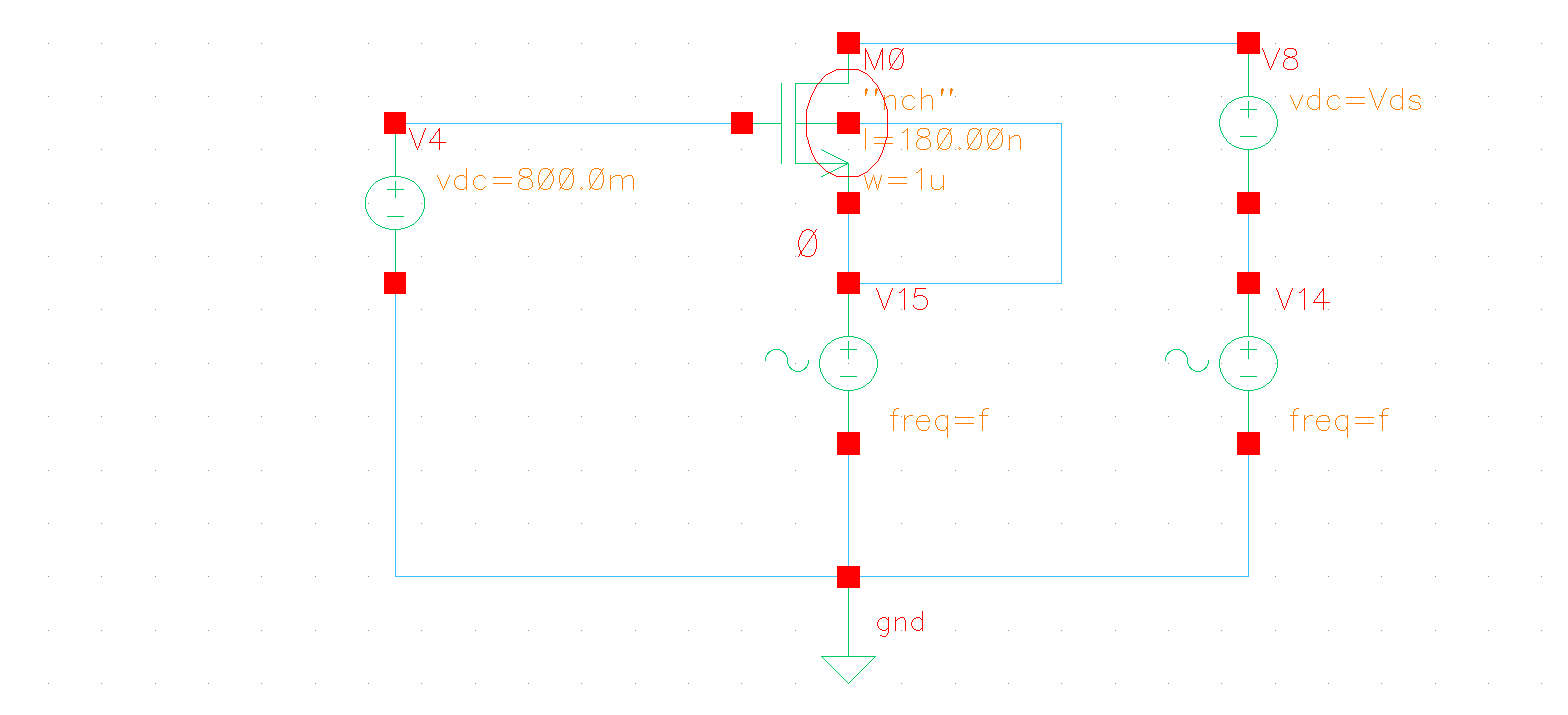
\includegraphics[width=7in]{1_ac_schematic.png}
\caption{Schematic to Simulate AC Operation}
\label{1_ac_schem}
\end{figure}

%\begin{figure}[H]
%\centering
%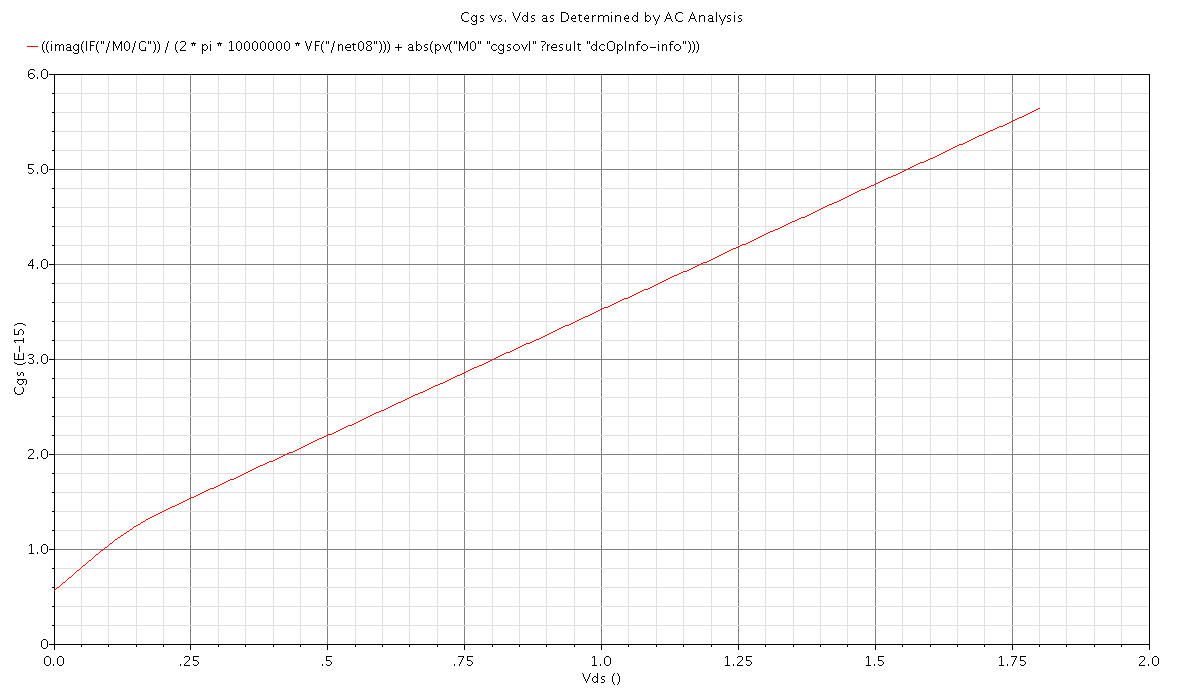
\includegraphics[width=5in]{1d.png}
%\caption{$C_{gs}$ vs. $V_{DS}$ as Determined by DC Operating Point Simulation}
%\label{1d}
%\end{figure}

\begin{figure}[H]
\centering
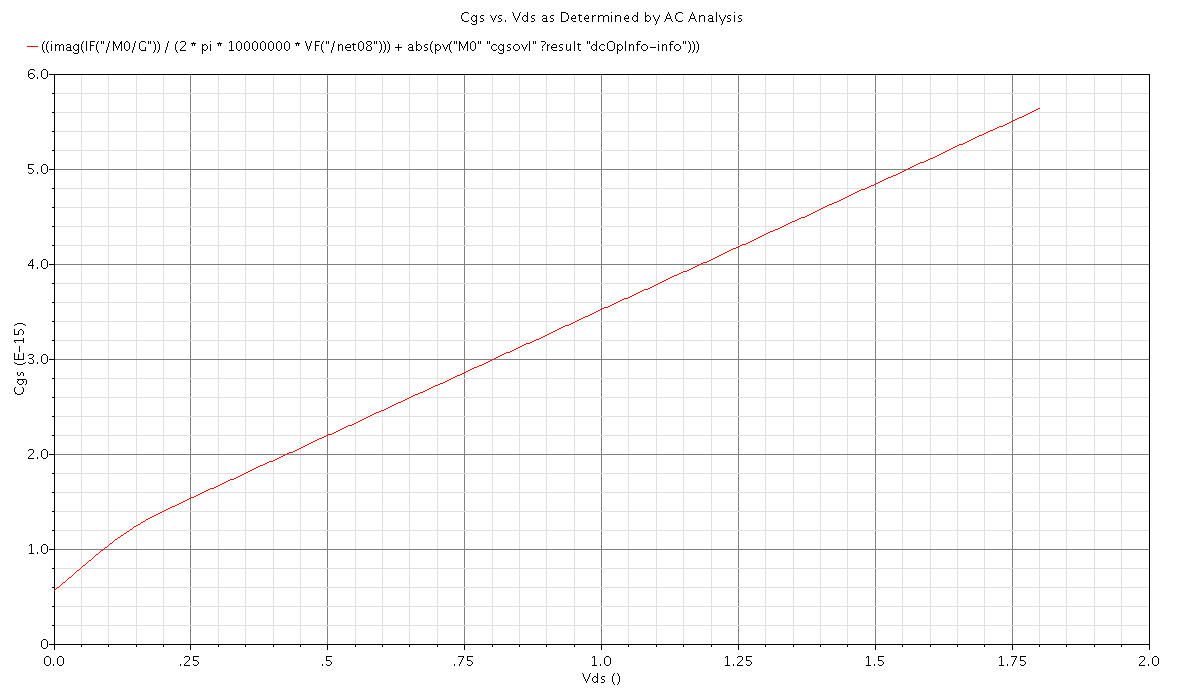
\includegraphics[width=5in]{1d.png}
\caption{$C_{gs}$ vs. $V_{DS}$ as Determined by AC Analysis}
\label{1d}
\end{figure}
\newpage

\subsection{$C_{gd}$}
To measure $C_{gd}$, I performed almost identical simulations to those of $C_{gs}$. However, to plot $C_{gd}$ using AC analysis, I applied an AC signal to the drain of the device instead of the source and simulated current into the gate. This has the same isolating effect but this time on $C_{gd}$ instead of $C_{gs}$. My plots can be seen in Figure \ref{1b} and Figure \ref{1e} (note that in these plots I also had to eliminate overlap capacitance which was acquired from the results browser. Similar to $C_{gs}$, $C_{gd}$ begins at $C_{OX}/2$, drops steadily, and then saturates to about 0F at $V_{DS-SAT}$.

\begin{figure}[H]
\centering
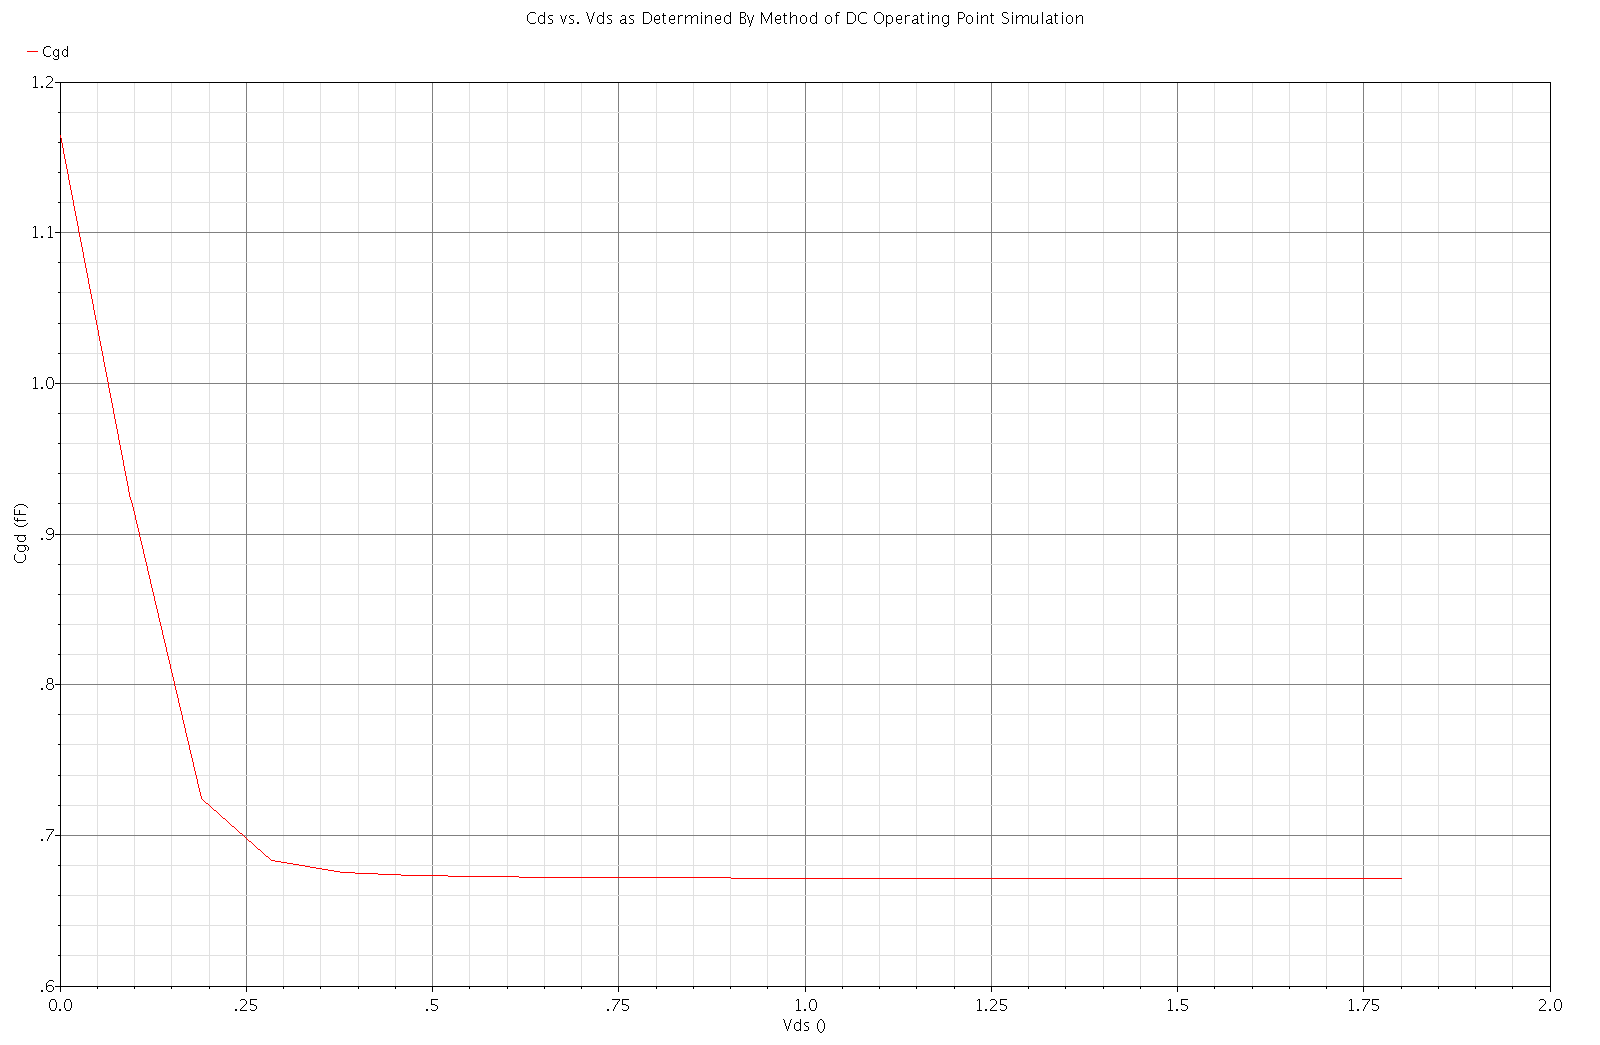
\includegraphics[width=5in]{1b.png}
\caption{$C_{gd}$ vs. $V_{DS}$ as Determined by DC Operating Point Simulation}
\label{1b}
\end{figure}

\begin{figure}[H]
\centering
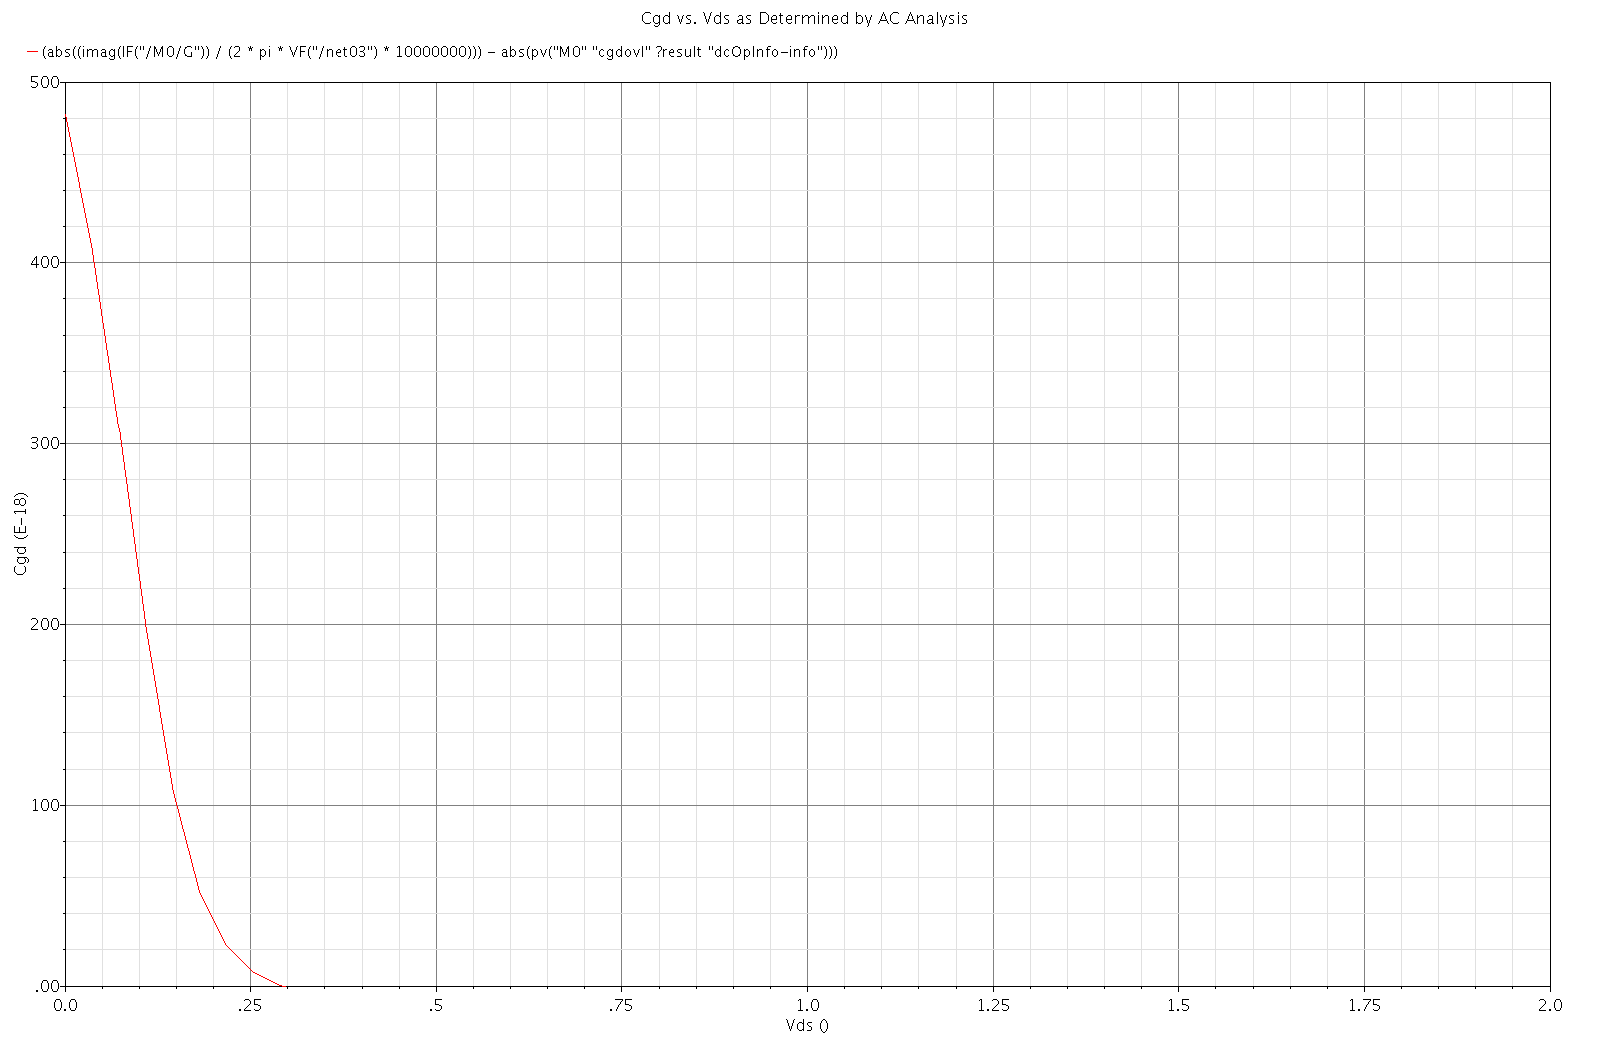
\includegraphics[width=5in]{1e.png}
\caption{$C_{gd}$ vs. $V_{DS}$ as Determined by AC Analysis}
\label{1e}
\end{figure}
\newpage

\subsection{$C_{db}$}
To measure $C_{db}$, I again performed similar DC and AC simulations on my circuit. To simulate the circuit for AC analysis I measured the current into the drain while actually applying an alternating signal to the body. My plots can be seen in Figure \ref{1c} and Figure \ref{1f}.

\begin{figure}[H]
\centering
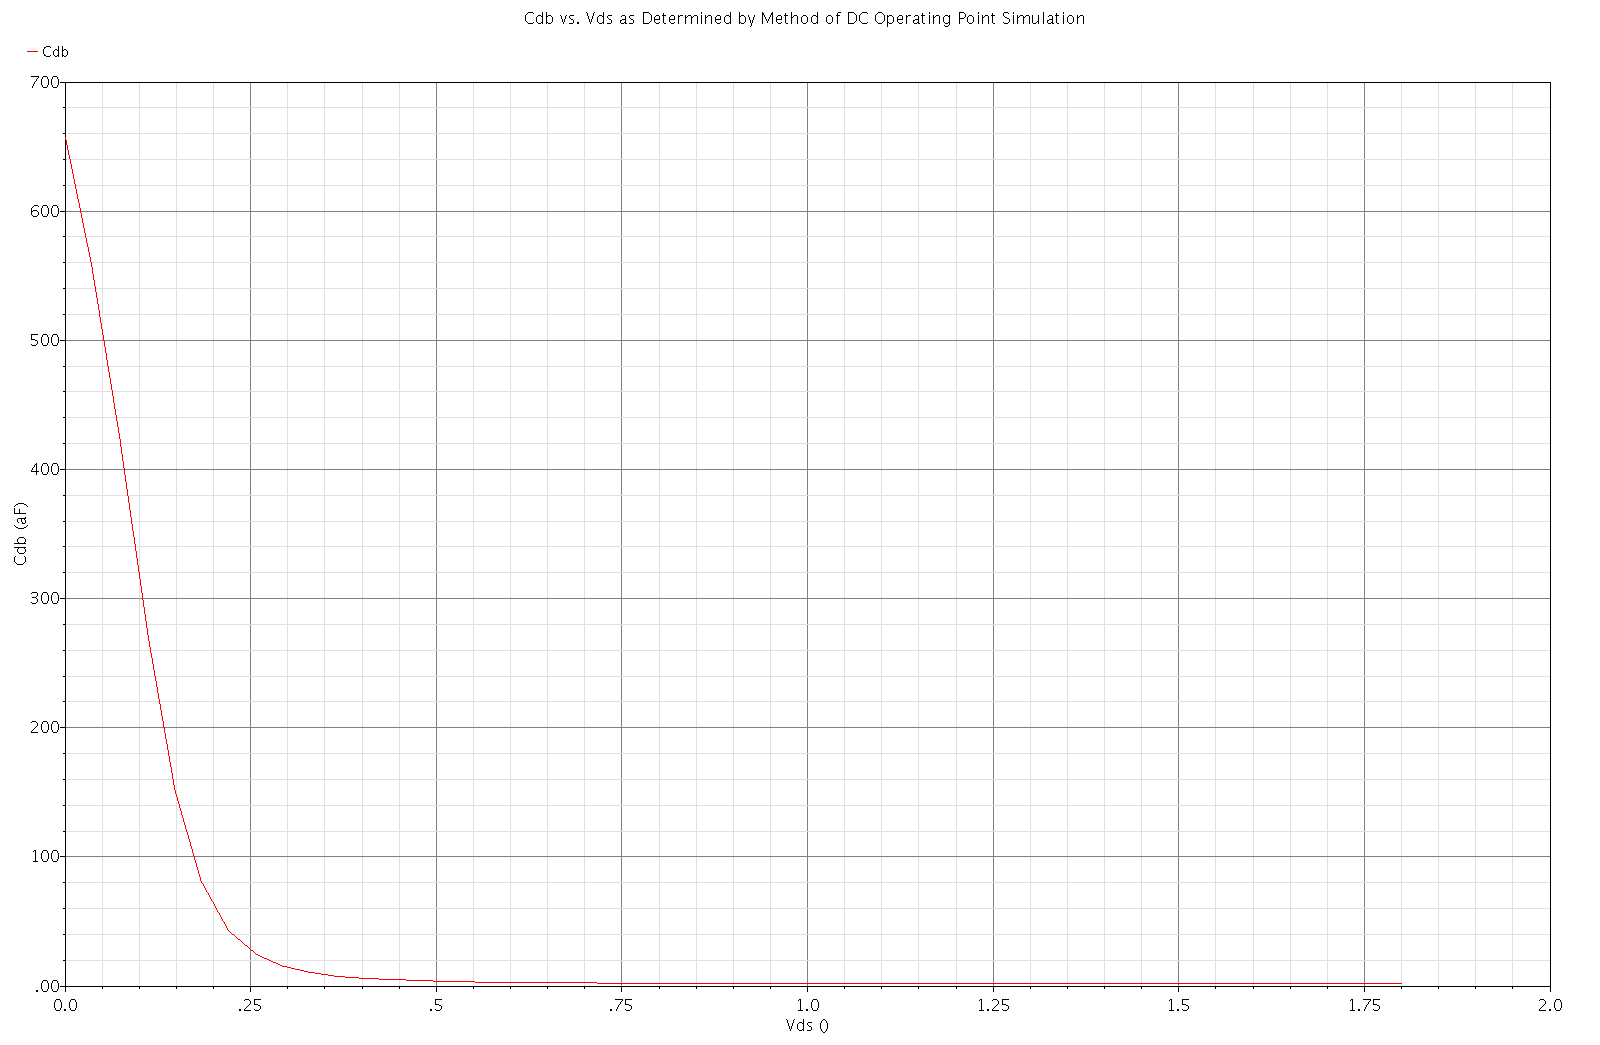
\includegraphics[width=5in]{1c.png}
\caption{$C_{db}$ vs. $V_{DS}$ as Determined by DC Operating Point Simulation}
\label{1c}
\end{figure}

\begin{figure}[H]
\centering
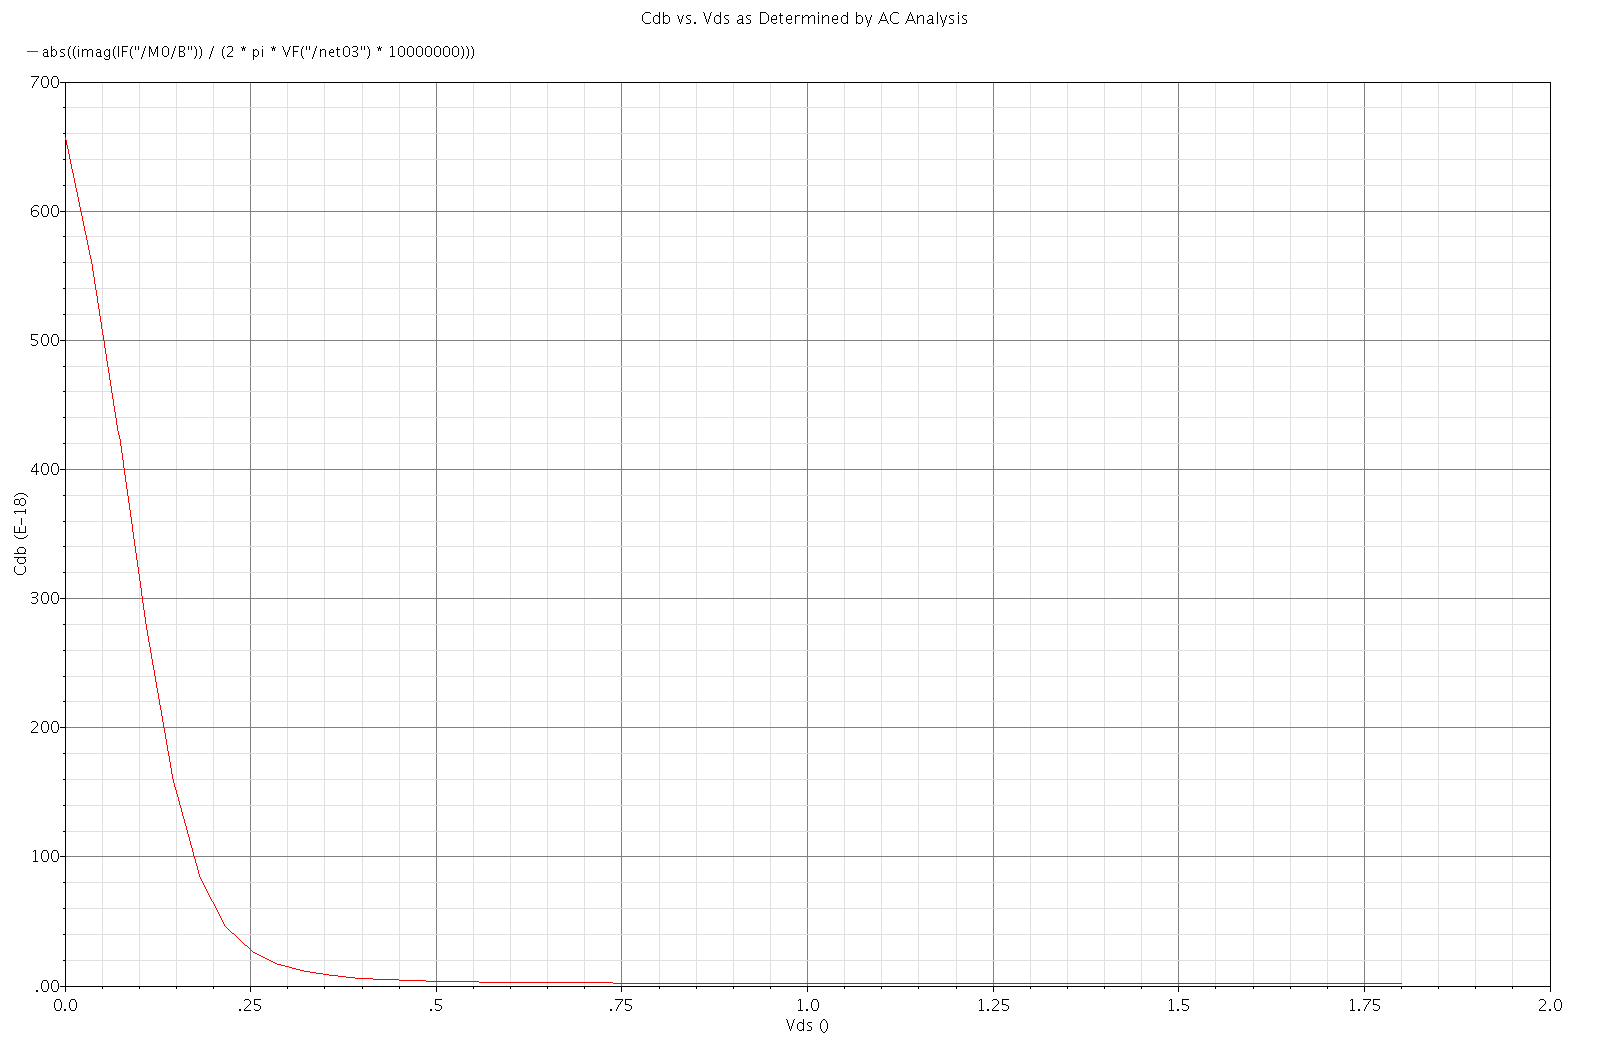
\includegraphics[width=5in]{1f.png}
\caption{$C_{db}$ vs. $V_{DS}$ as Determined by AC Analysis}
\label{1f}
\end{figure}
\newpage

\section{Problem 2: Basic Amplifiers}
\subsection{Common-Source}
For the first part of this problem, I designed a common source amplifier and all associated biasing circuitry. I began by placing my amplifier device as well as unsized placements of my current mirror devices. In order to achieve the maximum output voltage swing, I knew my goal was to set $V_{DS}$ of my amplifier device to approximately 0.9V (halfway between ground and $V_{dd}$). This also would ensure my device to stay in saturation. To achieve this voltage, I sized my current mirror devices appropriately until I observed $V_{DS} = 935.6mV$. Next I chose a value of $V_{GS}$ of 0.7V to bring the device into strong inversion. Because it was readily available from my previous design efforts, I simply connects the gate of my amplifier device to a node of my biasing circuit through a resistor. This brought my $V_{GS}$ to 574.1mV which was acceptable for my purposes. My final design step was to add a small signal source which I connected to the gate of my amplifier device through a large isolating capacitor. The capacitor prevents my small signal source from affecting the biasing of my amplifier. I noted that after the design was complete, $I_{DS}$ of my amplifier device was $17.38\mu A$. My final topology can be seen in Figure \ref{cs_schem}.

My next step was to analyze the performance of my circuit as three PVT corners. In the typical case (tt: typical corner, $27^oC$, $V_{dd} = 1.8V$, my low frequency gain was 32.61dB. In the best case (ff: fast corner, $-20^oC$, $V_{dd} = 2.0V$), my low frequency gain was 32.68dB. In the worst case (ss: slow corner, $85^oC$, $V_{dd} = 1.6V$), my low frequency gain was 29.41dB. This was the most steady performance across PVT variations I could achieve. Frequency response plots of these three cases can be seen in Figure \ref{cs_tt}, Figure \ref{cs_ff}, and Figure \ref{cs_ss} respectively.

\begin{figure}[H]
\centering
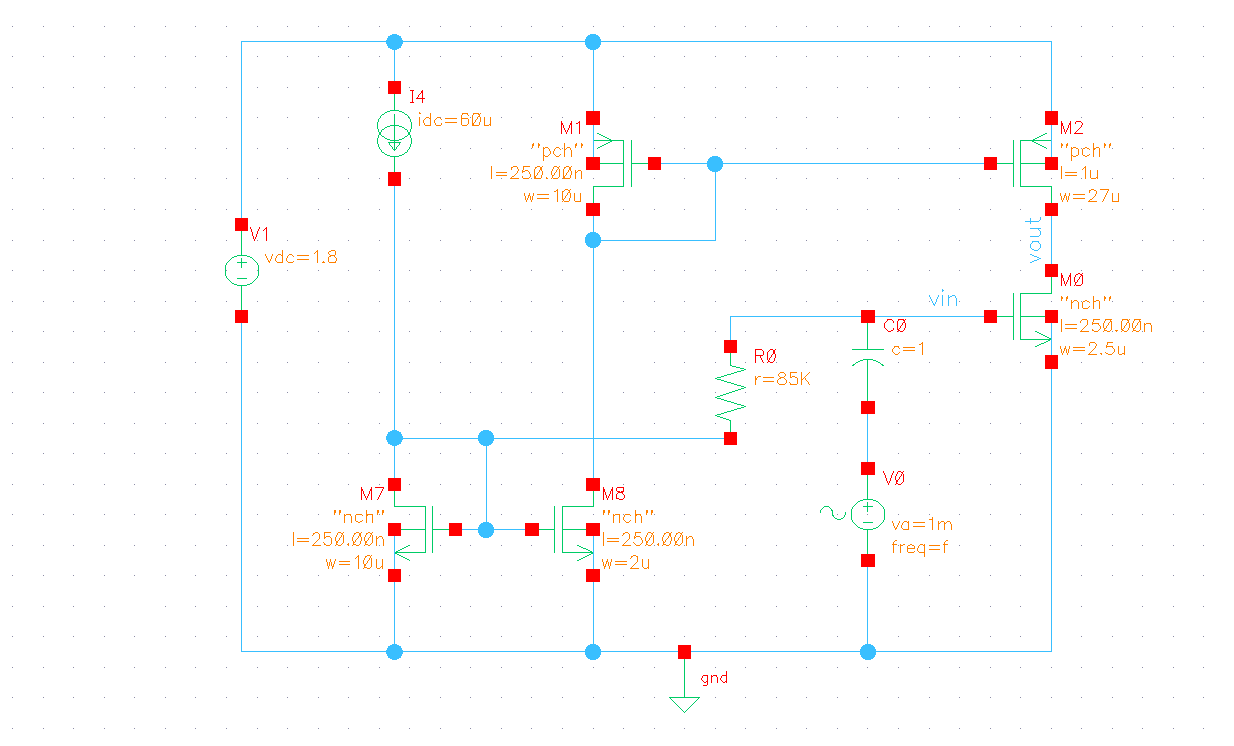
\includegraphics[width=7in]{2_cs_schematic.png}
\caption{Schematic of Common Source Amplifier and Associated Biasing Circuitry}
\label{cs_schem}
\end{figure}
\newpage

\begin{figure}[H]
\centering
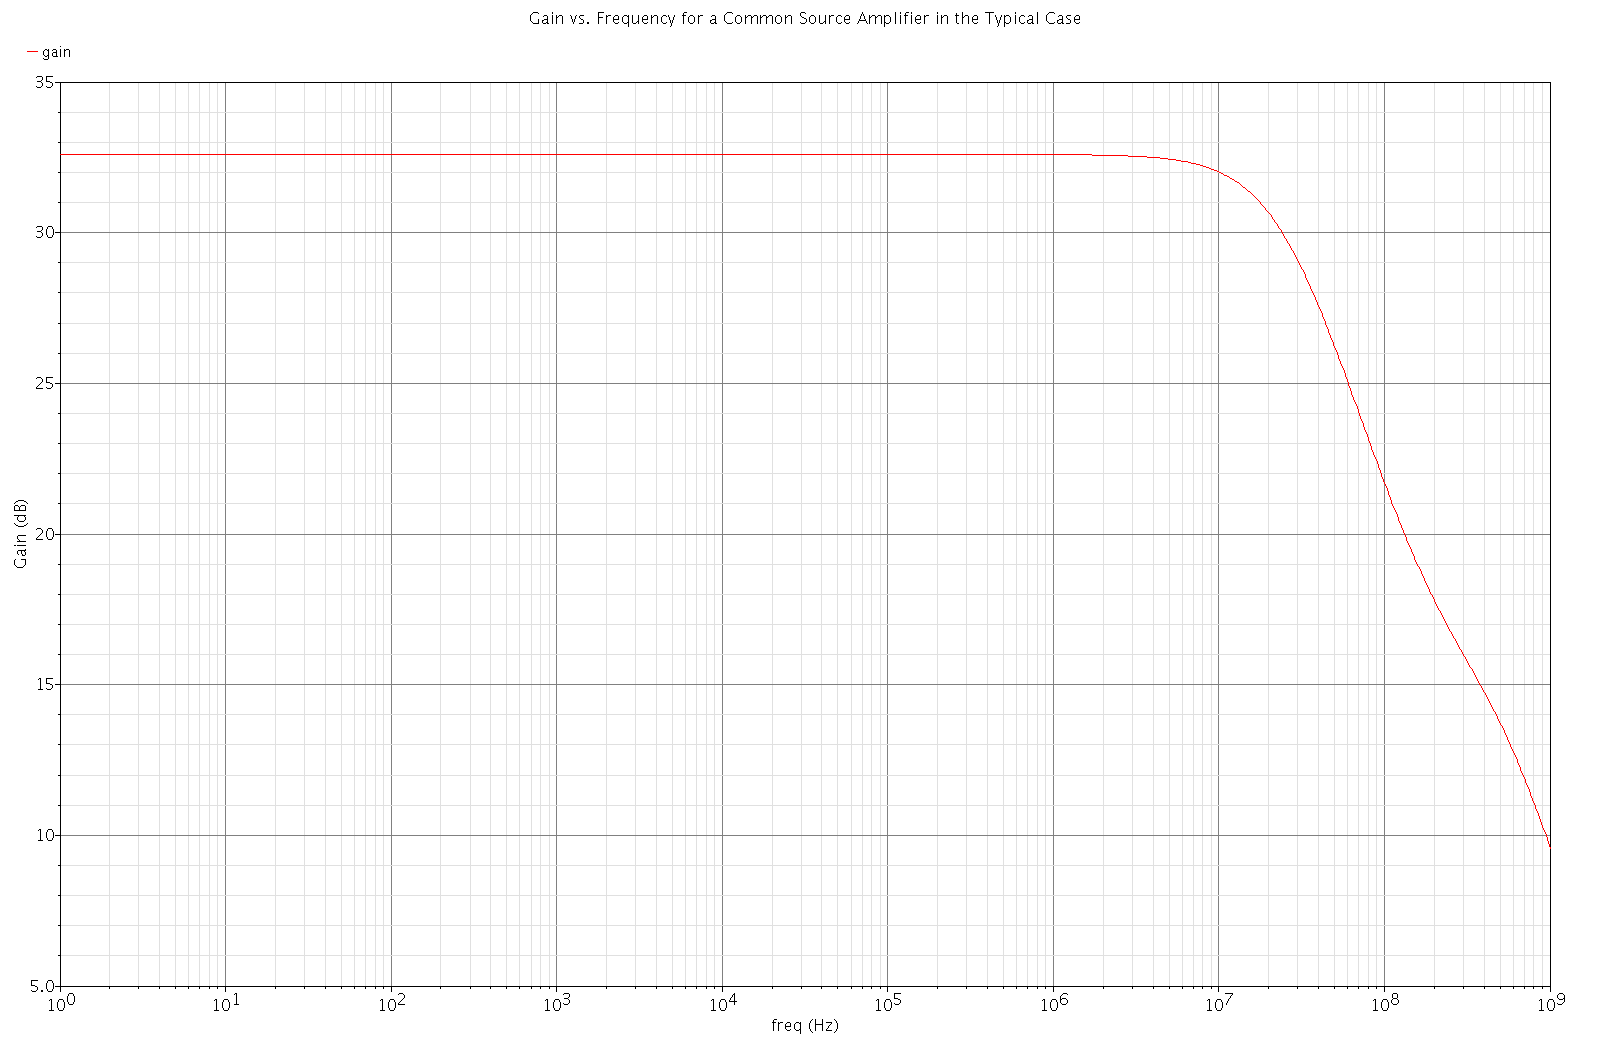
\includegraphics[width=5in]{2_cs_gain_tt.png}
\caption{Frequency Gain of Common Source Amplifier in the Typical Case}
\label{cs_tt}
\end{figure}

\begin{figure}[H]
\centering
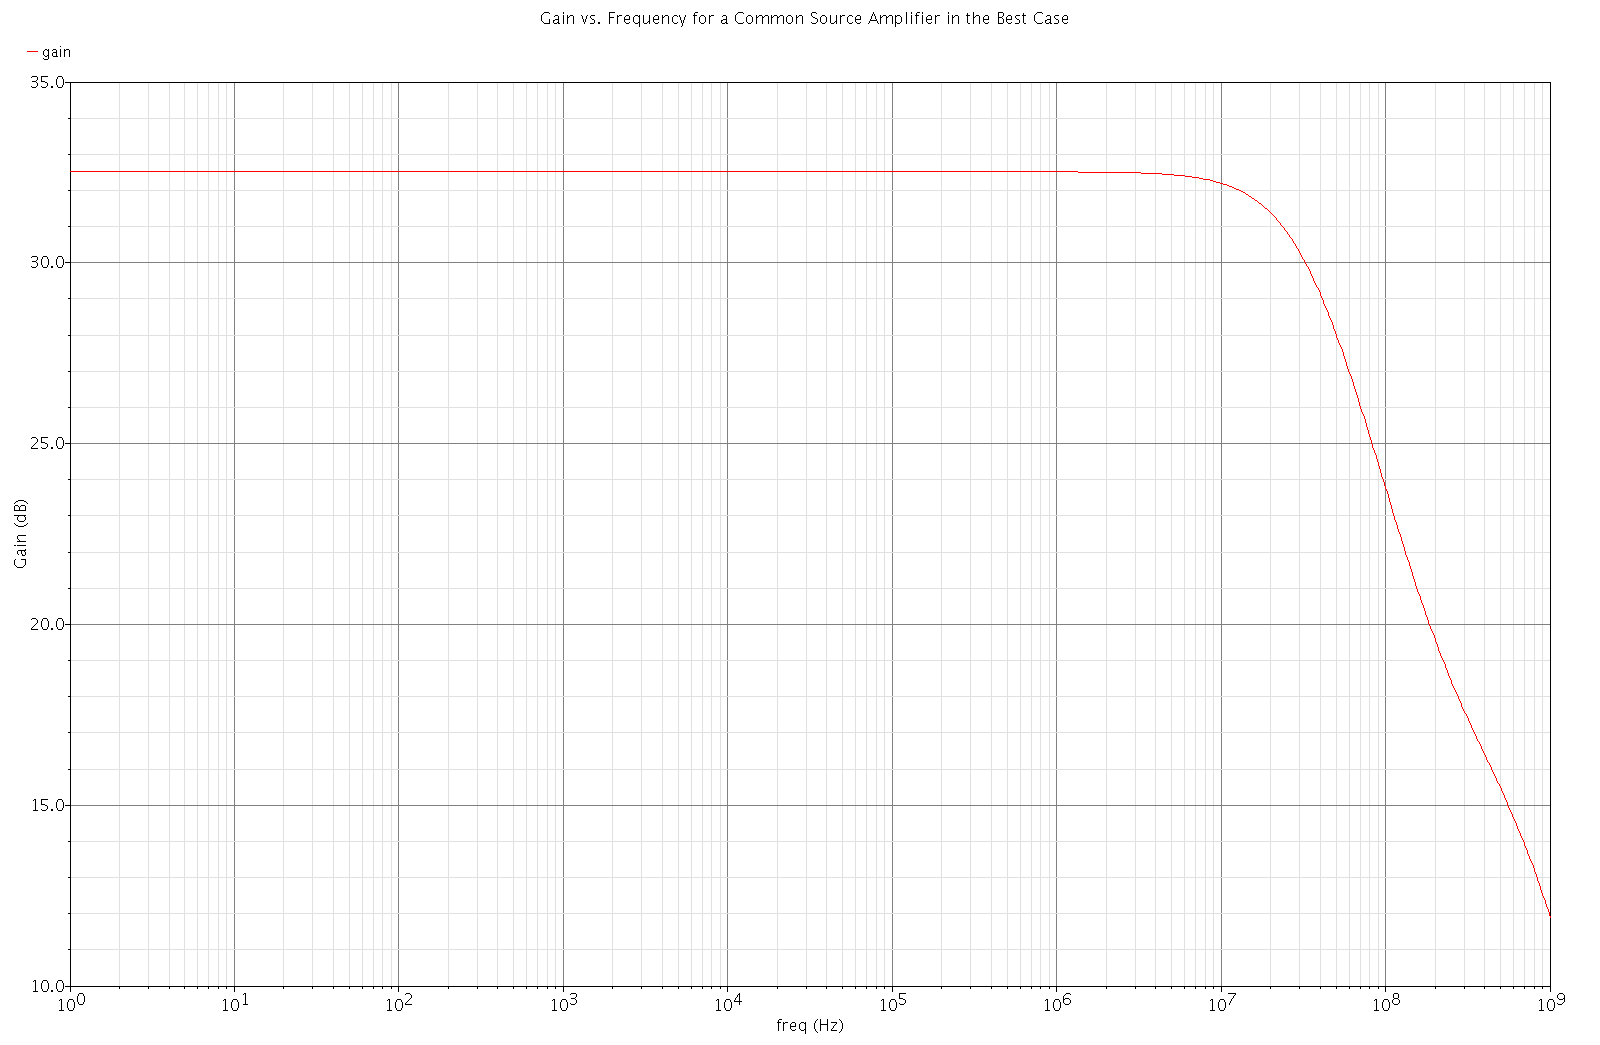
\includegraphics[width=5in]{2_cs_gain_ff.png}
\caption{Frequency Gain of Common Source Amplifier in the Best Case}
\label{cs_ff}
\end{figure}

\begin{figure}[H]
\centering
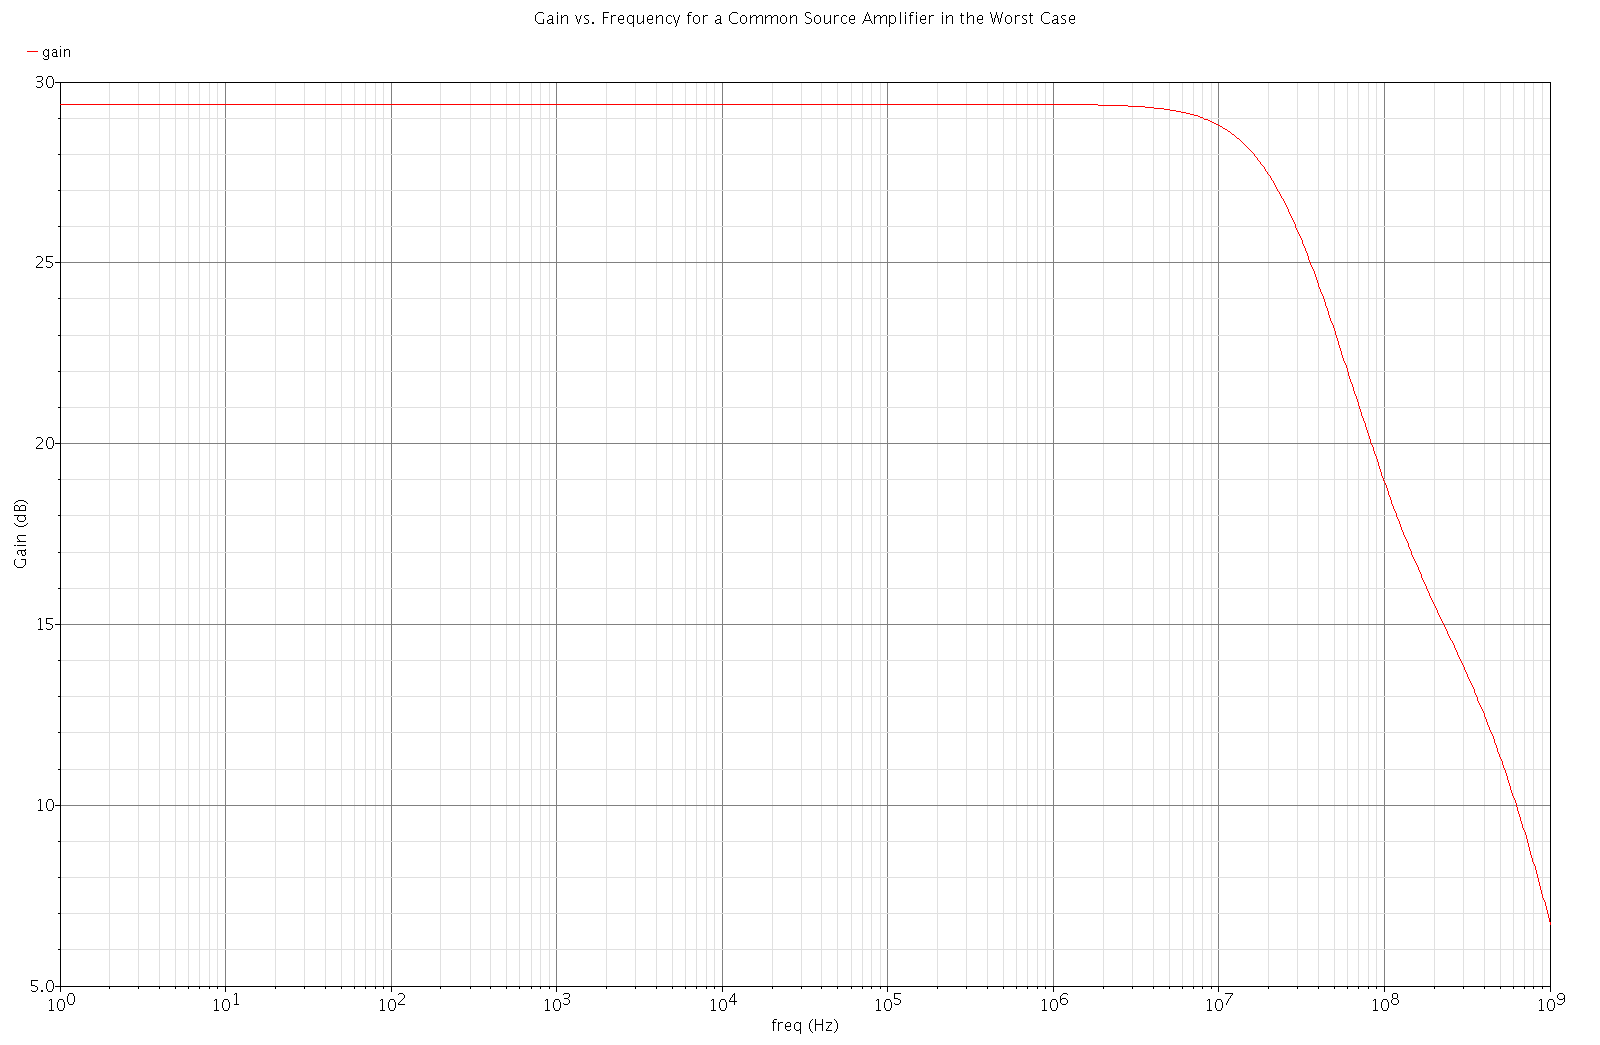
\includegraphics[width=5in]{2_cs_gain_ss.png}
\caption{Frequency Gain of Common Source Amplifier in the Worst Case}
\label{cs_ss}
\end{figure}

My final performance analysis task was to find the maximum input and output voltage swing. To do this I applied a small signal to the gate of the amplifier device at 1MHz and varied its amplitude. I plotted various transient responses on AC input voltage amplitudes between $20mV_{pp}$ and $50mV_{pp}$. As can be seen in Figure \ref{cs_tran}, the output begins to distort for larger amplitudes in the range. To determine the exact input voltage amplitude corresponding to -1dB of distortion, I used the calculator to plot an AC transfer function ($v_{out}$ vs. $v_{in}$). On this same plot, I also plotted a perfectly linear response if the amplifier had a gain of 31.61dB (-1dB). This can be seen in Figure \ref{cs_lin}. The intersection of these two curves shows the maximum input and output voltages (note that the plot shows amplitude from AC ground, not peak-to-peak). My final value of maximum input voltage for linear operation was $v_{in} = 36.56mV_{pp}$ with a corresponding output value of $v_{out} = 1.374V_{pp}$.

\begin{figure}[H]
\centering
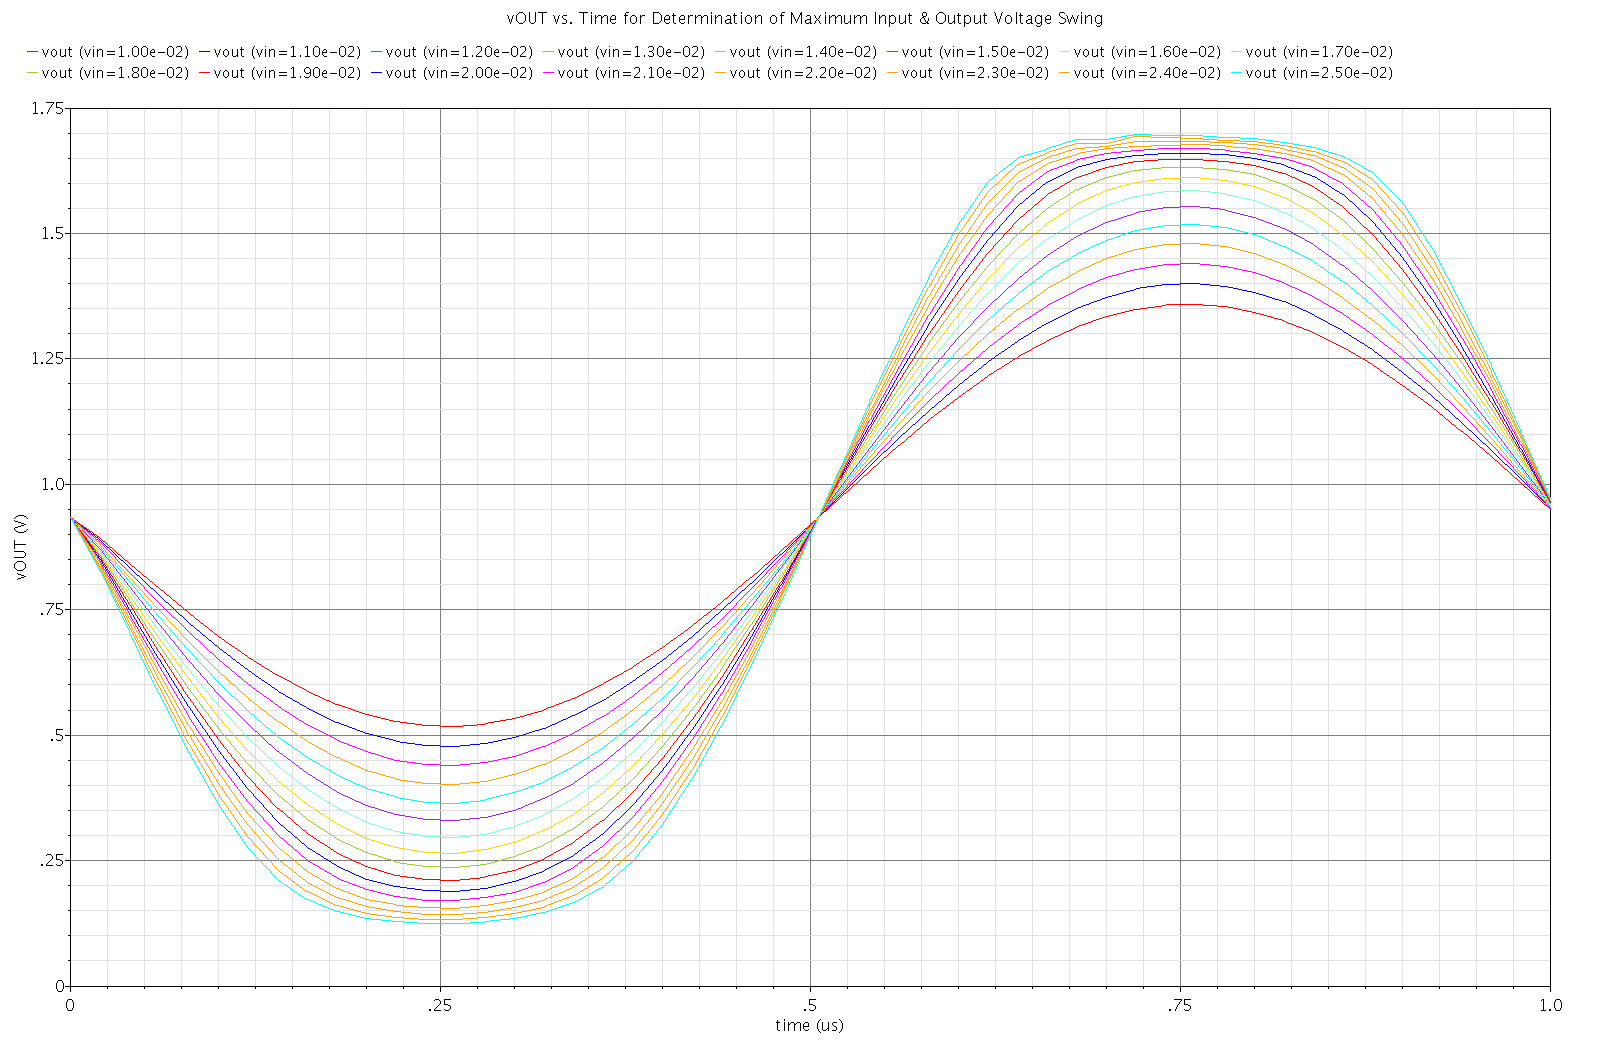
\includegraphics[width=5in]{2_cs_transient.png}
\caption{Transient Response of Output Voltage for Various Input Voltage Amplitudes}
\label{cs_tran}
\end{figure}

\begin{figure}[H]
\centering
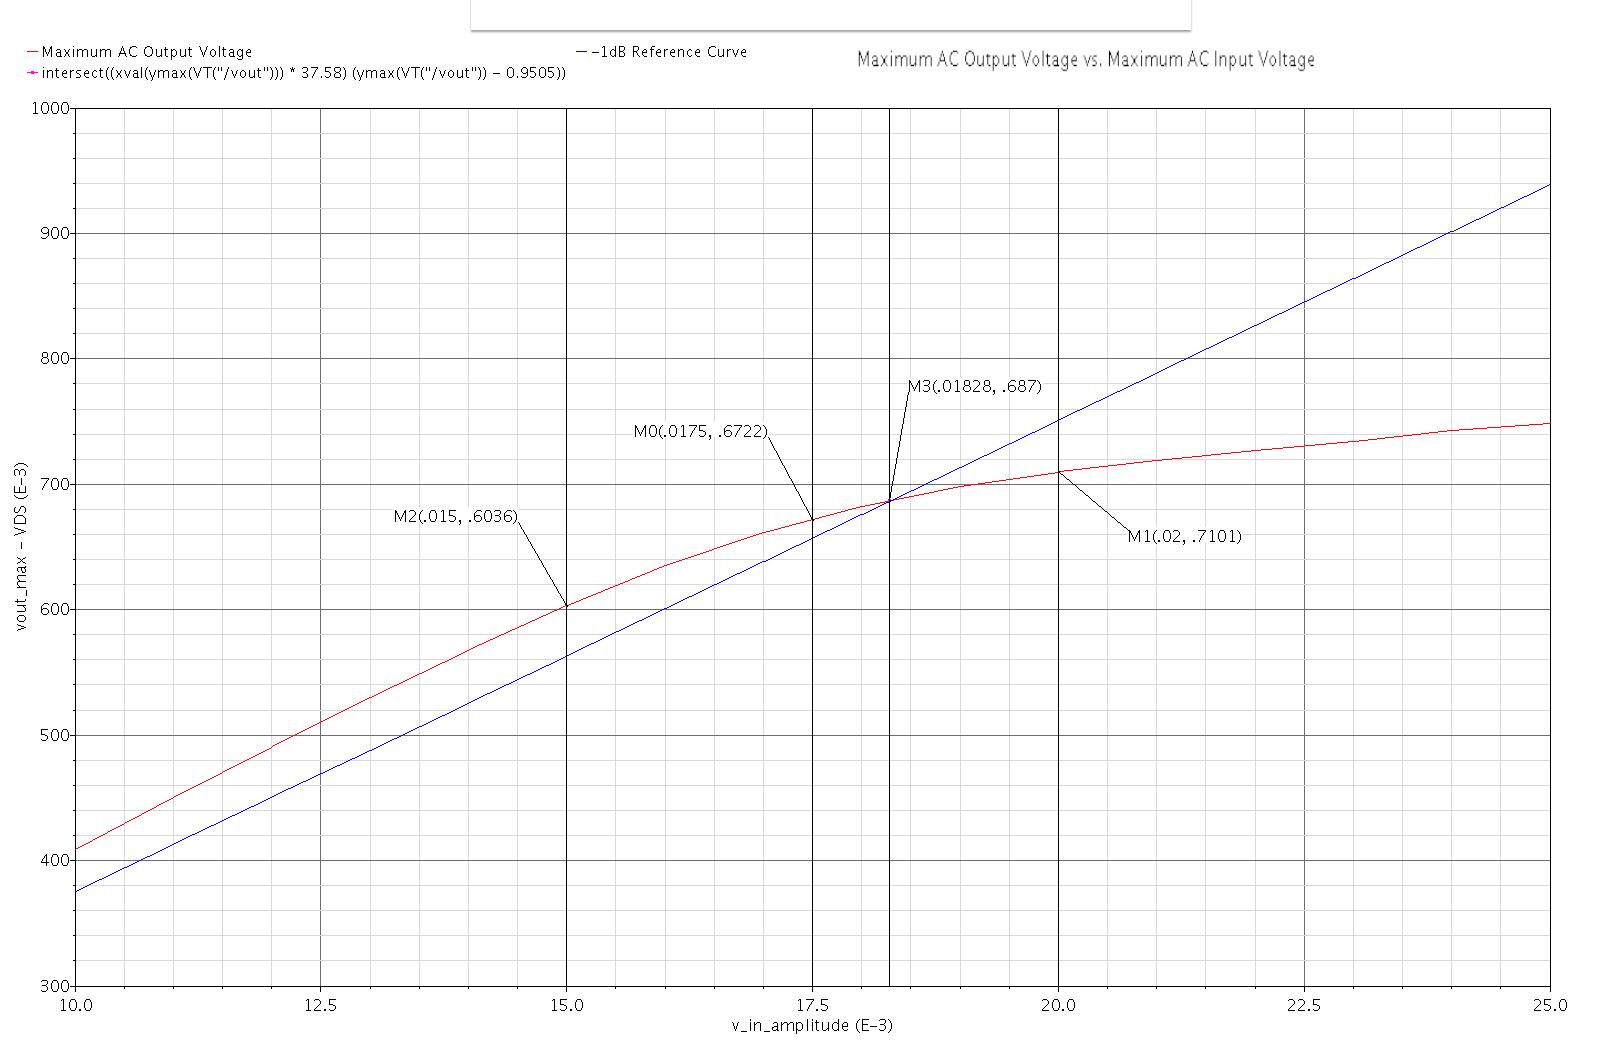
\includegraphics[width=5in]{2_cs_linearity.png}
\caption{AC Transfer Function of The Amplifier for Various Amplitudes with the -1dB Curve for Reference}
\label{cs_lin}
\end{figure}

\end{document}
